Logs are leveraged by developers to record useful information during the execution of a system. Logs are recorded during various development activities such as bug fixing~\cite{ConsoleLogs,JGLouMining,QFuanomaly}, load test analysis~\cite{Automatic}, monitoring performance~\cite{Yuan} and for knowledge transfer~\cite{IanWCRE}.
Logging can be done through the use of log libraries or more archaic methods such as \textsl{print} statements. Every log contains a textual part, which provides information about the context, a variable part providing information about the event and a log level, which shows the verbosity of the logs. An example of a log is shown below where info is the logging level, \textsl{Testing Connection to Host Id} is the context information and \textsl{host}, which is the variable part, provides information about the logging context.
\hypobox{LOG.info( ``Testing Connection to Host Id:" + host);}

The unified format of logs has lead to the development of many log processing tools such as \textsl{Splunk}~\cite{carasso2012exploring}, \textsl{Xpolog}, \textsl{Logstash}~\cite{xu2013detecting} and in-house tools. For example in Figure~\ref{fig:ExampleOfLogChange_LPA} we see that developers remove the time take for completing an event. This can effect log processing tools which rely on that information for other activities. Tools like Salsa~\cite{TanSalsa}, log-enhancer~\cite{Yuan}, chukwa~\cite{chukwa} 	are designed to diagnose as well as improve logging in software systems. These tools can be effected by such changes to logging statements and the data lost is not recoverable.


%These log processing tools are used to generate information for capacity planning of large-scale systems~\cite{hassan2008industrial,nagappan2009efficiently}, to monitor system health~\cite{bitincka2010optimizing} or to detect abnormal system behavior~\cite{JiangICSM2008}. These tools rely heavily on the log messages themselves and require continuous maintenance when the format or content of logs are changed.

\begin{figure}[tb]
\centering
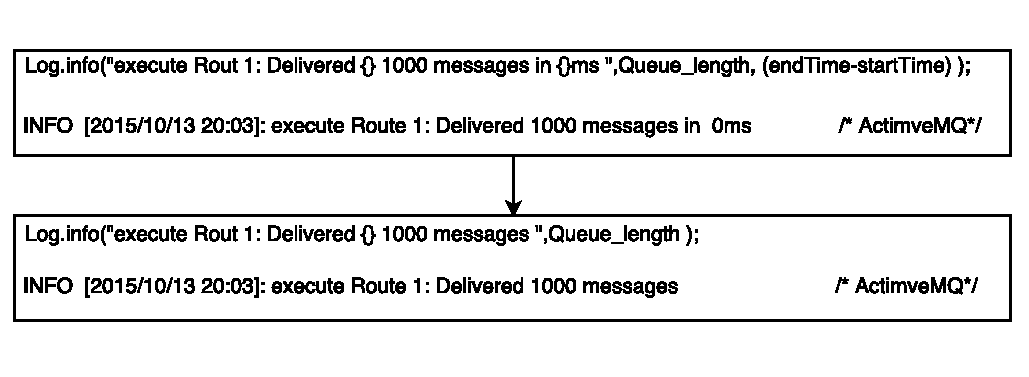
\includegraphics[width=1\columnwidth]{ExampleOfLogChange_LPA}
\caption{Modification of a logging statement}
\label{fig:ExampleOfLogChange_LPA}
\end{figure}



Research shows that only 40\% of the logs at execution level stays the same across releases and the impact of 15-80\% of the log changes can be minimized through robust analysis of the code changes~\cite{IanWCRE}. These log changes can affect the log processing tools which heavily depend on them and maintenance cost will be high. In this paper, we track the changes made to logs across multiple releases in four studied open source systems. In order to get a better understanding of the log changes we focus our research on the following RQ's.\\

% and use the data to answer the following research questions.

\textbf{RQ1:} \textbf{How much do logs change over time and why do the changes occur?}

Based on our quantitative analysis of the studied systems we identify three categories of change frequency in logs. If a log is changed more than four times we categorize it as \textsl{`Frequently Changed'}, if it has one to three changes, it is categorized as \textsl{`Changed'} and if there are no changes made we categorize it as \textsl{`Never Changed'}. We find that in our studied systems, 20-80\% of the logs are changed at least once throughout the lifespan. 

%We find developers change logs for four main reasons namely:`change of log level', `text modification', `variable modification' and `log relocation'.\\ 
% We find that only \textsl{Hadoop} has 60\% of log statements in the \textsl{`Never Changed'} category.In all other projects we find that \textsl{`Changed'} is majority ranging between 20\% - 68\% in CloudStack. We find that \textsl{`Frequently changed'} ranges between 1\% - 13\% in the four subject systems and is the least among the three categories. These results show that logs are not stable and there is need to study the stability of log statements in large subject systems.



\textbf{RQ2:} \textbf{Can code, log and developer metrics help in explaining the stability of logs?}

 We find that code, log and developer related metrics help in building models which can predict which logs are more likely to change in the future. We use the data from three dimensions namely, code, log and developers. Our \textsl{random forest} achieved an accuracy of 89\% to 93\% in all studied systems with recall of 76\% to 92\%, when predicting which logs have higher likelihood of getting changed. We also identify significant metrics from each dimension, that affect the stability of logs. We find several metrics (e.g., developer experience, source lines of code, \# of comments, log text length) are strong predictors in predicting if a log will change in the future. 
 
 
 Our results show that code, log and developer related metrics can help in identifying unstable logs in our studied systems. This can help in reducing the effort needed in the maintenance of log processing applications, as system maintainers can flag the logs that have the potential of being changed in subsequent releases and track them. 
 
The rest of this paper is organized as follows. Section~\ref{Methodology} presents the methodology for gathering and extracting data for our study. Section~\ref{studyresults} presents the case studies and the results to answer the two research questions. Section~\ref{related} describes the prior research that is related to our work. Section~\ref{threats} discusses the threats to validity. Finally, Section~\ref{conc} concludes the paper.
 
 
% However, as these tools are not scalable for all companies and systems, companies prefer in house development or customization of these tools for their specific purposes. 